\documentclass[11pt,a4paper,twoside,titlepage]{scrbook}
\usepackage[utf8]{inputenc}
\usepackage[ngerman, english]{babel}
\usepackage[pdfborder={0 0 0}]{hyperref}
\usepackage{amsmath}
\usepackage{amsfonts}
\usepackage{amssymb}
\usepackage{graphicx}
\usepackage{geometry}
\usepackage{tikz}
\usepackage{amsthm}
\usepackage{algorithmic}
\usepackage{algorithm}
\usepackage{float}
\usepackage{caption}
\usepackage{subcaption}
\usepackage{mathtools}
\usepackage{float}
\usepackage{comment}
\usepackage[section]{placeins}


\clubpenalty=1000
\widowpenalty=1000

\theoremstyle{definition}
\newtheorem{definition}{Definition}[section]
\newtheorem{lemma}{Lemma}
\newtheorem{theorem}{Theorem}
\newtheorem{corollary}{Corollary}




\begin{document}
	
	\frontmatter

	%----- TITLE PAGE -----
	
	\begin{titlepage}
		%\noindent\makebox[\linewidth]{\rule{\paperwidth}{0.4pt}}
	
		\begin{tikzpicture}[remember picture, overlay]
		\node [anchor=north east, inner sep=0pt]  at (17.9,2)%(current page.north east)
			{
\includegraphics[height=3.5cm]{figures/tu-bs_logo.jpg}};
		\end{tikzpicture}
		
		\centering
		\vspace{5cm}
		{\scshape\huge Bachelor Thesis\par}
		\vspace{1.5cm}
		{\Huge\bfseries Motion Planning for Reconfigurable Magnetic Modular Cubes in the 2-Dimensional Special Euclidean Group \par}
		\vspace{3cm}
		{\huge Kjell Keune\par}
		\vfill
		Institut für Betriebssysteme und Rechnerverbund\\
		\vfill
		
		Supervised by\par
		Prof. Dr. Aaron T. Becker\par
		
		\vfill
		
		% Bottom of the page
		{\large \today\par}
	\end{titlepage}
	
	\cleardoublepage
	
	% statement of originality
	\thispagestyle{plain} % no header
	\vspace*{7cm}
	\centerline{\bfseries Statement of Originality}
	\vspace*{1em}
	\noindent
	This thesis has been performed independently with the support of my supervisor/s.
	To the best of the author's knowledge, this thesis contains no material previously
	published or written by another person except where due reference is made in the text.
	
	\par
	\bigskip\noindent Braunschweig, \today \par
	\vspace*{10mm}
	\hfill\hrulefill
	\cleardoublepage
	
	
	\chapter*{Aufgabenstellung / Task Description}


\paragraph{Deutsch:}
\begin{otherlanguage}{ngerman}
	Um spezifische Aufgaben besser zu bewältigen, lassen sich modulare, rekonfigurierbare Roboter zu größeren Strukturen zusammensetzen und wieder auseinandernehmen.
	Magnetic-modular-cubes sind skalierbare Einheiten, bei welchen Permanentmagneten in einen würfelförmigen Körper eingebettet sind.
	Diese Einheiten zählen als rekonfigurierbare Roboter, obwohl sie selber keine Logik oder Stromversorgung beinhalten.
	Stattdessen lassen sich diese durch ein externes, gleichmäßiges und sich zeitlich änderndes Magnetfeld steuern.
	Durch diese Steuerung können die magnetic-cubes auf der Stelle gedreht oder durch pivot-walking nach rechts und links bewegt werden.
	Obwohl sich das Magnetfeld auf alle Einheiten gleichermaßen auswirkt, kann durch Kollision mit der Arbeitsflächenbegrenzung eine Änderung der Anordnung bewirkt werden.
	Befinden sich zwei magnetic-cubes nah genug beieinander können sich diese durch die Permanentmagneten miteinander verbinden und so Polyominos als größere Strukturen aufbauen,
	welche auf die gleiche Weise wie einzelne cubes gesteuert werden können.
	Frühere Arbeiten betrachteten das "tilt-model", bei welchem sich Strukturen jeder Größe mit gleicher Geschwindigkeit in ganzzahligen Schritten und mit ausschließen 90° Drehungen bewegen lassen.
	
	Herr Keunes Aufgabe in dieser Bachelorarbeit ist es, einen motion-planner für die beschriebenen magnetic-cubes zu entwerfen, welcher mit beliebigen Positionen und Rotationen umgehen kann.
	Dabei ist es erforderlich, eine Simulationsumgebung zu schaffen, welche das Verhalten der magnetic-cubes repliziert.
	Es soll ein lokaler motion-planner entwickelt werden, um zwei Polyominos an gewünschten Kanten zu verbinden.
	Dieser local-planner soll Heuristiken und optimale Bewegungsabläufe mit möglichst wenig Schritten realisieren.
	Ebenfalls soll dieser global eingesetzt werden, um Bewegungsabläufe zu finden, die gewünschte Polyominos aus einer zufällig gegebenen Startkonfiguration erzeugen.
	Ein interessantes Ergebnis wird es sein, zu sehen, wie gut Probleminstanzen dieser Art in der Realität gelöst werden können und welche Parameter die gravierendsten Auswirkungen auf die Schwierigkeit von motion-planning Problemen haben. 
	
\end{otherlanguage}

\newpage

\paragraph{English:}
Reconfigurable modular robots can dynamically assemble/disassemble to better accomplish a desired task.
Magnetic modular cubes are scalable modular subunits with embedded permanent magnets in a 3D-printed cubic body.
These cubes can act as reconfigurable modular robots, even though they contain no power, actuation or computing.
Instead, these cubes can be wirelessly controlled by an external, uniform, time-varying magnetic field.
This control allows the cubes to spin in place or pivot walk to the left or right direction.
%Rotating the magnetic field can make the cubes spin in place.
%The cubes can pivot walk by first lifting their magnetic north (or south) end up, then rotating the cubes about the end touching the workspace, and then then lowering the cube back onto the workspace.   
Although the applied magnetic field is the same for each magnetic modular cube, collisions with workspace boundaries can be used to rearrange the cubes.
Moreover, the cubes magnetically self-assemble when brought in close proximity of another cube, and form polyominoes, which can be controlled the same way as single cubes.  
%These polyominoes can also pivot walk and rotate in place.
Related work has considered the “tilt model,” where similar cubes and polyominoes move between integer positions, all move at the same speed, and only rotate by 90 degree steps.

In his thesis, Mr. Keune's task is to design a motion planner for magnetic cubes that can assume arbitrary positions and orientations in the workspace.
This requires designing a simulation environment that replicates the behavior of magnetic cubes.
He will design local planners for moving two polyominoes to assemble at desired faces.
Designing the local planner includes heuristics and computing optimal motion plans that minimize the number of steps.
The local planner will be used to search for global planning sequences to generate desired polyominoes from a given starting configuration.
One exciting outcome will be studying how well instances can be solved in practice and analyzing which parameters have the most significant effect on the difficulty of the motion planning problem. 
	
	%---------------------
	\chapter*{Abstract}
Abstract \cite{Becker2014_SP}
\cite{LaValle2006}
\cite{Becker2022}
	
	\tableofcontents
	
	%% Remove listoffigures or listoftables if not needed!
	\listoffigures
	
	%\listoftables
	
	\mainmatter
	
	\chapter{Introduction}
\label{chap:intro}

Self-assembling modular parts forming bigger structures is a well-known concept in nature.
Most functionalities of living organisms follow this principle \cite{bishop2005}.
DNA, for example, has the ability to self-replicate by using differently shaped proteins that combine themselves in various ways.
At larger sizes, these cells can be combined to assemble tissue, organs and even whole organisms.
Complex structures, like proteins, can be assembled and disassembled depending on the task they should accomplish at a given point in time. 
Using self-reconfiguring robot swarms in such a way has promising applications in the future.
Biomedical applications could be targeted drug delivery or drug screening \cite{sitti2015}, or a robot swarm could be used for milliscale and microscale manufacturing \cite{pelrine2016}.

Designing robots at these small sizes faces challenging problems.
Equipping each robot with its own sensors, actuation-system, connection-system and power supply seem infeasible, in terms of the miniaturization required and power-limitations \cite{white2007}.

Therefore, the use of external global control, effecting every robot in the workspace with the same torque and force, is a promising solution \cite{white2007}.
Using robots with embedded permanent magnets, has all the desired effects.
Robots can be controlled by an external magnetic field and also connect to each other without any internal power supply and for sensing an external camera can be used \cite{saab2019}.

One example for magnetically controlled robots are the magnetic modular cubes by Bhattacharjee et al.\ \cite{Bhattacharjee2022}, which are the subjects of this thesis.
We will look at the difficulties and problems that occur, when assembling structures with magnetic modular cubes in the 2-dimensional special Euclidean group \(SE(2)\), the space of rigid movements in a 2-dimensional plane.

\section{Related Work}

Continuous motion planning is a crucial subject in the field of robotics.
The goal is to find a path from the initial state of a robot to a desired goal state, by performing actions which the robot is capable of.
The movement may result in collision with static obstacles and with other robots, but the objects may not overlap.
The state of the system is also called a configuration.
All possible configurations one or multiple robots can be in is defined as the configuration-space.
Motion planning complexity is often exponential in the dimension of the configuration space \cite{LaValle2006}.
Increasing the number of robots and/or possible actions, increases the dimension of the configuration space.
It is difficult to engineer algorithms that explore these huge configuration-spaces and provide continuous path from the initial to the goal configuration, or report failure, if the goal is not reachable.
Decades of research has been done on motion planning.
The textbooks \cite{LaValle2006} and \cite{Mueller2019} offer a great overview and also explain a lot of important concepts in detail.

When working with configuration-spaces that are uncountable infinite, like the special Euclidean group, one concept that has been successful for many robotics problem is sample-based motion planning.

By taking samples, you can reduce the planning problem from navigating a configuration space to planning on a graph, but you might lose possible solutions.
Algorithms like that are not complete anymore, but by using a good sampling technique you can get arbitrarily close to any point.
Ways of sampling include random sampling being probabilistically complete or using a grid with a resolution that is dynamically adjustable resulting in resolution completeness.
After sampling, conventional discrete planning algorithms can be applied \cite{LaValle2006}.

One state-of-the-art sampling-based approach uses rapidly-exploring random trees (RRT).
This method tries to grow a tree-shaped graph in the configuration space by moving into the direction of randomly chosen samples from already explored configurations. That way the space gets explored uniformly without being too fixated on the goal configuration \cite{lavalle1998,lavalle2001}.

When working with multiple robots, the interaction of robots with each other becomes important.
One interesting idea is that single robots can connect to form bigger structures.
This is referred to as self-assembly and E. Winfree \cite{winfree1998} proposed the abstract Tile Assembly Model (aTAM) in the context of assembling DNA.
In this model, particles can have different sets of glues and connect according to certain rules regarding the glue type.
However, he considers this process as nondeterministic, so there is no exact instruction on how to assemble a desired structure.

One model more related to the magnetic modular cubes is the Tilt model from Becker et al.\ \cite{Becker2014_SP}.
In the Tilt model, all tiles move into one of the cardinal directions until hitting an obstacle.
Different variations of the model include moving everything only one step, or the maximally possible amount.
It offers a solution for motion planning problems when robots are controlled uniformly by external global control inputs.

In \cite{Becker2014_SP} it is shown that transforming one configuration into another, known as the reconfiguration-problem, is NP-hard.
Caballero et al.\ \cite{caballero2020} also researched complexity of problems regarding the Tilt model.
Following work \cite{Becker2014} also proves that finding an optimal control sequence, minimizing the number of actions, for the configuration-problem is PSPACE-complete.
Furthermore, research is done on designing environments in which the Tilt model can be used to accomplish certain tasks.
In particular, Becker et al.\ \cite{Becker2014} create connected logic gates that can evaluate logical expressions.

More on the side of self-assembly, in \cite{Becker2020} the construction of desired shapes using the tilt model is researched.
It presents a method that can determine a building sequence for a polyomino by adding one tile at a time, considering the rules of Tilt.
Also examined are ways of modifying the environment to create factories that construct shapes in a pipeline by repeating the same global control inputs.
Shapes can be constructed more efficiently by combining multi-tiled shapes to an even bigger structure.
One article considering the construction with so-called sub-assemblies is proposed by A. Schmidt \cite{Schmidt2018}.

Most recently, Bhattacharjee et al.\ \cite{Bhattacharjee2022} developed the magnetic modular cubes.
These robots contain embedded permanent magnets and have no computation or power supply.
Instead, they are controlled by an external time-varying magnetic field and are able to perform various actions.
Most importantly, they can rotate in place or use a technique called pivot walking to move either left or right.
The magnets also act as glues and allow the cubes to perform self-assembly.
Although it is theoretically possible to assemble 3-dimensional structures, most research was done by only connecting cubes in two dimensions.
Since all cubes are the same size, the assembled 2-dimensional shapes can be represented as polyominoes.
An enumeration was done on the amount of possible polyominoes that can be created by cubes with different magnet configurations \cite{Lu2021}.

By limiting the controls to only 90 degree turns and assuming a uniform pivot walking distance for all structures per step, magnetic modular cubes follow rules similar to the Tilt model.
Following these limitations, a simple discrete open-loop motion planer was developed, that explores a finite configuration-space and lists all the possible polyominoes that can be created from an initial configuration \cite{Bhattacharjee2022}.

One interesting paper from Blumenberg et al.\ \cite{blumenberg2023} explores the assembly of specific target polyominoes in arbitrary environments, when cubes obey the tilt model in a discrete setting.
He provides different algorithmic approaches using various distance heuristics and a solution making use of RRTs.

Lu et al.\ \cite{Lu2023} are working on establishing closed-loop control for magnetic modular cubes by using computer vision-based feedback of the workspace.
The used motion planner is still working in a discrete setting, but can assembly specific target shapes, while handling collision events of estimated continuous motion.


\section{Contribution}

We provide more information about the general framework of magnetic modular cubes on which this thesis relies in \autoref{chap:prelim}.

In \autoref{chap:local} we develop a local planner that is connecting two magnetic modular cube structures at desired faces.
We do this with a closed-loop algorithm to account for all types of collision events.
The resulting local plans are not optimal, but follow heuristics for minimizing the cost of movements.
The local planner focuses more on reducing planning time. 

The local planner works with our magnetic modular cube simulator presented in \autoref{chap:sim}.
This 2D-physics simulator aims to replicate the behavior of magnetic modular cubes accurately, while still being efficient enough to be used for motion planning.
The simulator does not assume discrete movement or limits rotations to a certain amount.

Based on the local planner we develop a global planning algorithm in \autoref{chap:global}, which provides a control sequence to assemble desired target structures.
The configuration-space is sampled by only considering connections between structures as local plans and using a specially constructed graph as a building instruction for target polyominoes.
The use of RRTs would be too inefficient, since we are working with a high fidelity simulation. 

Results evaluating our global planner are presented in \autoref{chap:results} and a conclusion with possible directions for future work is given in \autoref{chap:conclusion}.
	\chapter{Preliminaries}
\label{chap:prelim}



\section{Magnetic Modular Cubes}

\begin{figure}
	\centering
	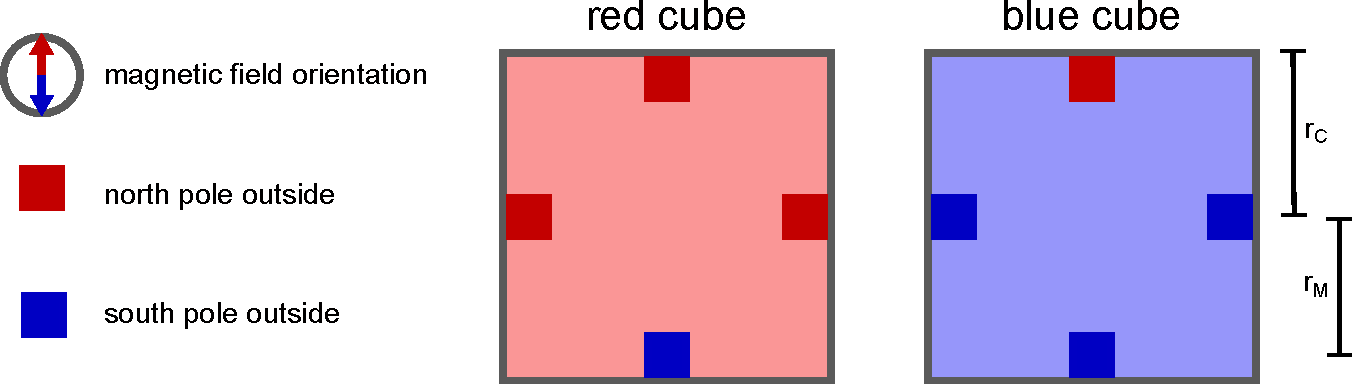
\includegraphics[width=0.75\textwidth]{figures/magnetic_cubes.pdf}
	\caption[Top-down view of the two magnetic modular cube types]{Simplified top-down view of the two magnetic modular cube types with their outward pointing magnet poles, illustrated as red and blue squares. Also visualizes the lengths $r_C$ and $r_M$ and the cardinal direction vectors of all cube faces.}
	\label{fig:magnetic_cubes}
\end{figure}

\begin{figure}
	\centering
	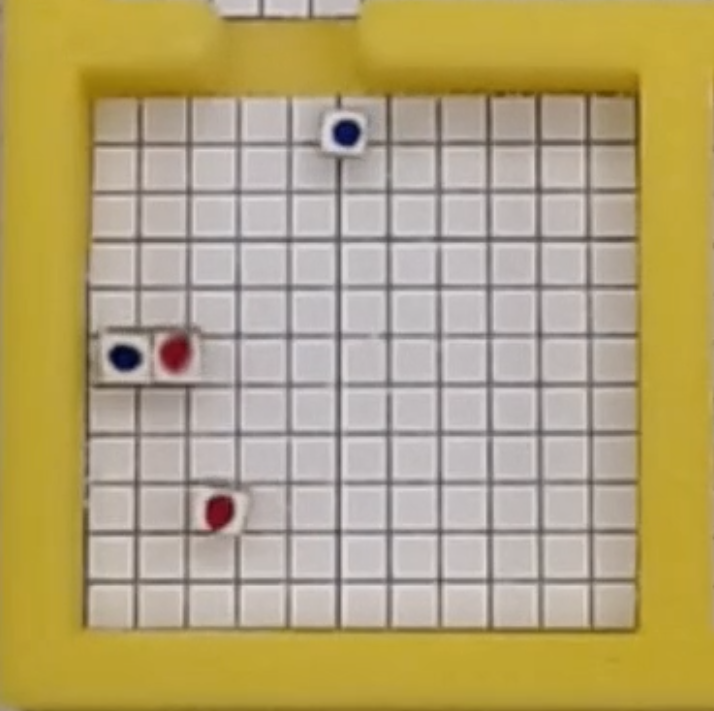
\includegraphics[width=0.5\textwidth]{figures/real_mmcs.png}
	\caption[Picture of magnetic modular cubes in real workspace]{Magnetic modular cubes with 2.8 mm edges in a real workspace. Picture was taken from a video made by A. Bhattacharjee showing the assembly of a four cube polyomino.}
	\label{fig:real_mmcs}
\end{figure}


The magnetic modular cubes are cube-shaped bodies embedded with permanent magnets on the four side faces.
The magnets have different orientations of their north and south pole. 
One pole is always pointing outward and the other straight to the center of the cube.
The magnet at the front face has its north pole pointing outwards and the magnet at the back its south pole.
These two magnets ensure that the cube is always aligned with the global magnetic field and this orientation holds true for both cube types.
The two other side faces must have the same outwards pointing pole, so that this axis does not provide a magnetic torque.

In fact, this is the reason a distinct definition of front, back and side is even possible.
Since the front is always pointing to the north pole of the magnetic field, we also call it the north face, or north edge in two dimensions, and all the other faces can also be called by their corresponding cardinal direction.
For each face we define a vector $\vec{e} \in \{ \vec{N},\vec{E},\vec{S},\vec{W}\}$ with $\lVert \vec{e} \rVert = 1$ pointing in the cardinal direction of the magnetic field.
For simplification we refer to magnets by their outwards pointing pole in further sections.

Furthermore, two different cube types are defined:
Either both side magnets point out their north pole, these cubes are called red cubes, or they point out their south pole, which is then called a blue cube.
\autoref{fig:magnetic_cubes} shows a top-down view of the two cube types with all the outwards pointing magnet poles.
A compass always shows the orientation of the magnetic field in our illustrations.

Magnetic Modular Cubes can be constructed in different sizes and ways. For more technical details and length measurements, we refer to the original paper \cite{Bhattacharjee2022}.
In \autoref{fig:real_mmcs} magnetic modular cubes with 2.8 mm edges can be seen in a real workspace.
Two important lengths that we use for planning and simulating are the cube radius $r_C$ and the magnet radius $r_M$ (also illustrated in \autoref{fig:magnetic_cubes}).
$r_C$ is one half-length of a cube face and $r_M$ is the distance from the center of the cube to the center of the magnet.



\section{Workspace and Configuration}

\begin{figure}
	\centering
	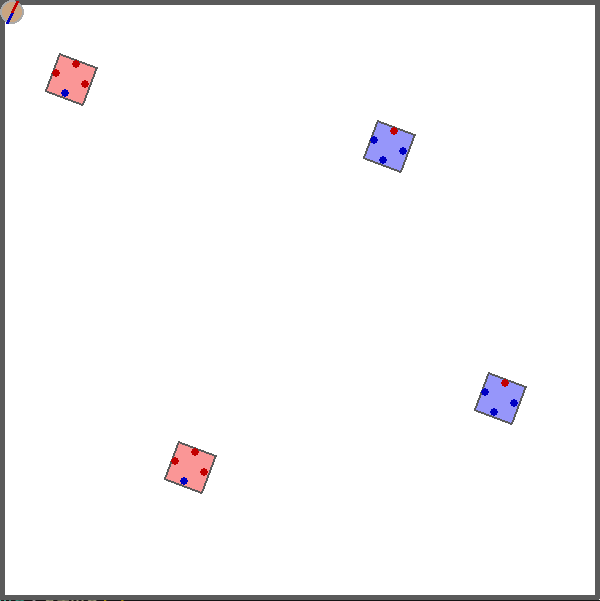
\includegraphics[width=0.45\textwidth]{figures/workspace_config.png}
	\caption[Workspace with a configuration of four magnetic modular cubes]{Rectangular workspace with a configuration of four magnetic modular cubes. All cubes have the same orientation as the magnetic field, indicated by the compass in the top-left corner.}
	\label{fig:workspace_config}
\end{figure}

Magnetic modular cubes could theoretically be placed and maneuvered on any 2-dimensional plane with numerous obstacles, as long as you can surround the workspace with a time varying magnetic field.
The magnetic field should be able to point in any direction specified by angles of latitude and longitude, so that the cubes can operate in all desired motion modes.
Because the motion planning problem of self-assembling target shapes in the special Euclidean group is hard enough without considering obstacles and arbitrary workspace shapes, this thesis limits itself to a rectangular workspace with no internal obstacles.
The workspace is bounded by surrounding walls, which are the only objects that could be considered as obstacles in classical motion planning.
However, we do not assume a fixed size, as long as the workspace stays finite and rectangular.

For planning we work in the configuration space of the 2-dimensional special Euclidean group $SE(2) = \mathbb{R}^2 \times \mathbb{S}^1$.
When only considering one cube, the group consists of the position in $\mathbb{R}^2$ and an orientation $\mathbb{S} = [0,2\pi)$ \cite{LaValle2006}.
When working with $n$ cubes, the dimension of our configuration space increases to $\mathbb{R}^{2n} \times \mathbb{S}^1$.
Note that we can still assume only one orientation for $n$ cubes, because we are working with a global magnetic field orienting all cubes the same way.
We assume that eventually all cubes align with the global magnetic field and only consider static configurations.
Future work could examine the dynamic configuration, which would enable faster motion planning, but a more complex planning problem.
\autoref{fig:workspace_config} shows a configuration with four cubes in the workspace.
It is irrelevant which exact physical cube is at which position as long as they are the same type, so switching the positions of the two red cubes in \autoref{fig:workspace_config} would lead to the same configuration as before.

\section{Polyominoes}
\label{sec:polys}

\begin{figure}
	\centering
	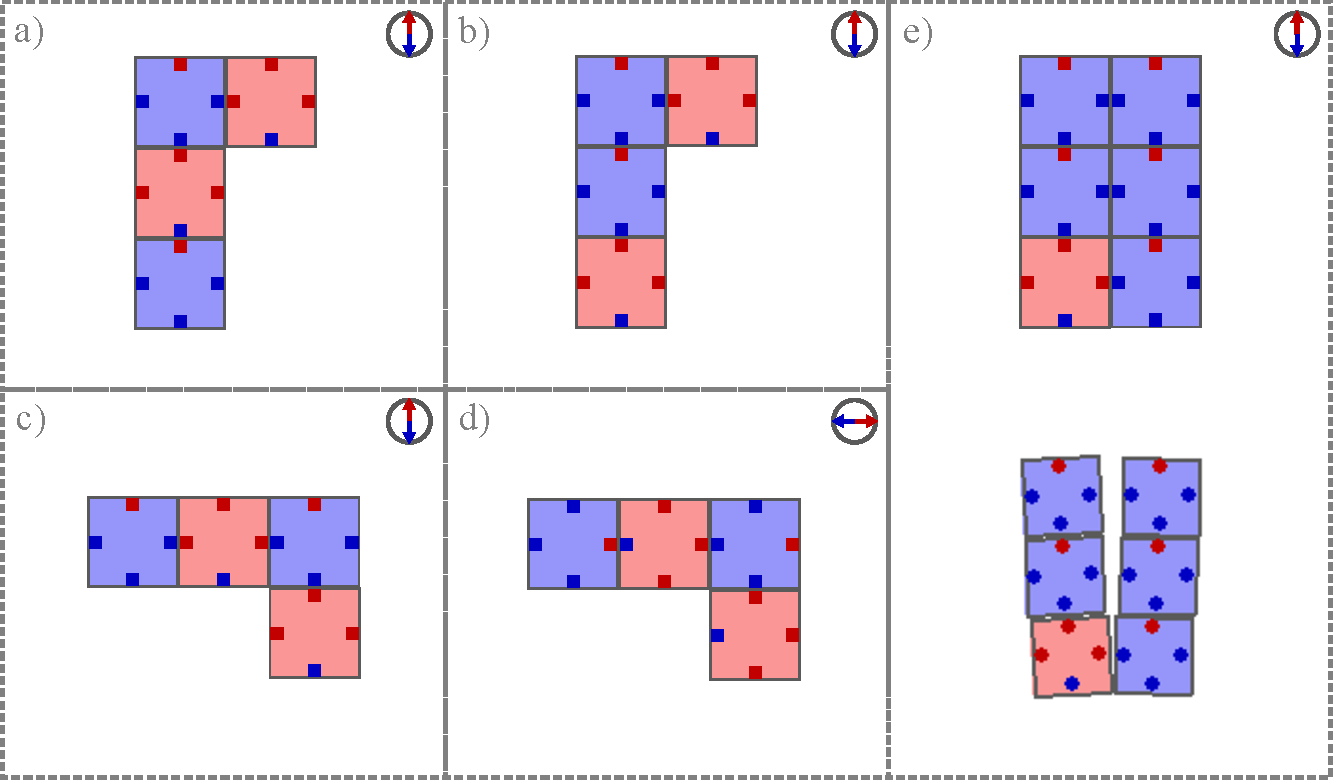
\includegraphics[width=0.65\textwidth]{figures/polyominoes.pdf}
	\caption[Examples of Polyominoes and their equality]{Examples of polyominoes and their equality. a) and d) are equal, only the magnetic field changed its orientation. a) and c) are not equal, they have the same shape, but it is rotated. a) and b) are also not equal because of different cube types in the same shape. e) shows an invalid polyomino in its grid representation (top) and how it behaves in the simulation (bottom).}
	\label{fig:polyominoes}
\end{figure}

The embedded magnets not only align the cube with the magnetic field, they also allow cubes to self-assemble into polyominoes.
Two cube faces can connect if their magnets have opposite polarities.
Because of this and the alignment with the magnetic field, cubes can either be connected at north and south faces, or east and west faces, if the cubes are not the same type.
A \textit{polyomino} is a set of uniformly sized cubes on a 2-dimensional grid.
Because we work with arbitrary positions and orientations the grid alignment does not hold true for multiple polyominoes in the workspace, but for each polyomino on its own the cubes can be represented in a local coordinate system with position $(x,y)$, $x,y \in \mathbb{Z}$ \cite{Lu2021}.

We consider \textit{fixed polyominoes}, meaning that two polyominoes are distinct if their shape or orientation are different \cite{Lu2021}.
The magnetic field always provides an orientation, so in \autoref{fig:polyominoes} a) and d) the polyominoes are equal, just the magnetic field is rotated.
Conversely, the polyominoes in \autoref{fig:polyominoes} a) and c) are the same shape but with a different rotation under the same magnetic field orientation, so they are not equal.
Furthermore, two polyominoes are only equal if all the cubes at equal positions are the same type.
The polyominoes in \autoref{fig:polyominoes} a) and b) are not equal because the cube types differ.
It is possible that a workspace contains multiple equal polyominoes.
In that case, we refer to them as being the same polyomino-type, instead of calling them equal, since it is important to differentiate between physical polyominoes with different positions.

The size of a polyomino is the number of cubes it consists of.
Because it is easier to view all structures in the workspace as a polyomino, single cubes are often referred to as trivial polyominoes with size 1.
Although it is not possible to connect cubes of same type at east and west faces, the magnetic modular cubes can assemble structures like the one shown in \autoref{fig:polyominoes} e).
The connection of the bottom two cubes is strong enough to hold the structure together, even though the four blue cubes on the top repel each other.
The resulting polyomino in its grid representation has two east-west connections between cubes the same type and is therefor marked as an invalid polyomino.


\section{Motion Modes}
\label{sec:motion}

\begin{figure}
	\centering
	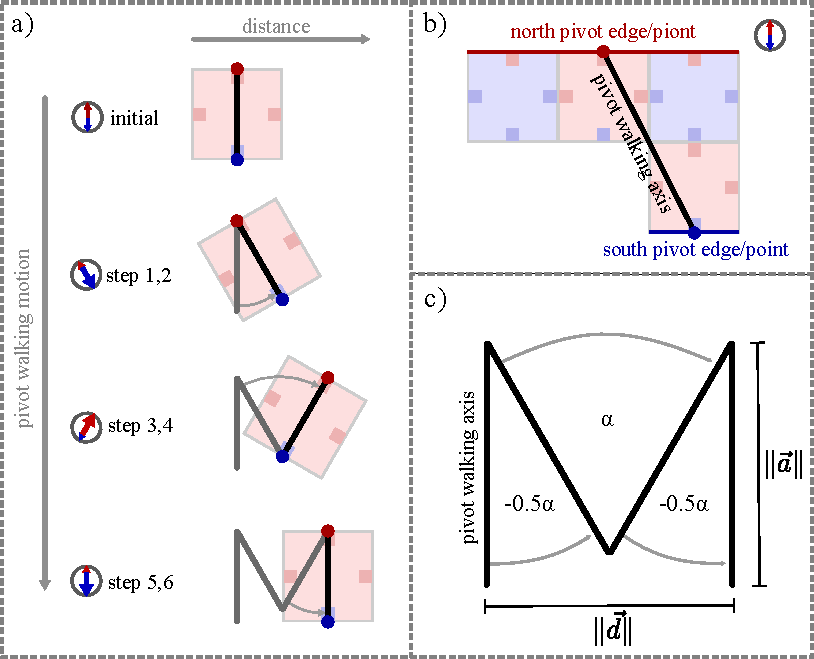
\includegraphics[width=0.80\textwidth]{figures/pivot_walking.pdf}
	\caption[Illustration of the pivot walking motion]{This figure describes the pivot walking motion in detail. a) shows the six pivot walking steps for a single red cube. You can see the orientation of the magnetic field (bigger arrow indicates elevation, so in step 1,2 the south pole is raised in the air). In b) an example polyomino with its pivot axis, edges and points is shown. c) illustrates the rotation of the pivot axis labeled with all the pivot walking parameters.}
	\label{fig:pivot_walking}
\end{figure}

In \cite{Bhattacharjee2022} three motion modes are presented. Rotation, pivot walking, and rolling.

If the magnetic field orientation lays in the plane of the workspace and rotates without any inclination the rotation is performed around the center of mass for all polyominoes and we consider this motion a normal rotation.

Rotating the magnetic field perpendicular to the workspace plane, cubes can roll forwards or backwards.
This rolling motion becomes problematic for self-assembly, because the top and bottom face of the cube, which contain no magnets, can become a side face.
Because rotation and pivot walking are sufficient to reach any position in the workspace, we do not consider rolling in our simulation and planning algorithms.

When elevating the magnetic field orientation by lifting up the south pole slightly, all polyominoes will pivot on the north face bottom edges of their most north-placed cubes.
Pulling up the north pole does the opposite. The polyominoes will pivot on the south face bottom edges of their most south-placed cubes.
The sum of all these cube edges is called the north or south pivot-edge and by keeping the magnetic field elevated and rotating around the normal vector of the workspace plane, the polyominoes will rotate around the center point of their pivot-edge.
This point is called the north or south pivot-point.
All these edges and points are illustrated in \autoref{fig:pivot_walking} b).


\paragraph{pivot walking:}

\begin{figure}
	\centering
	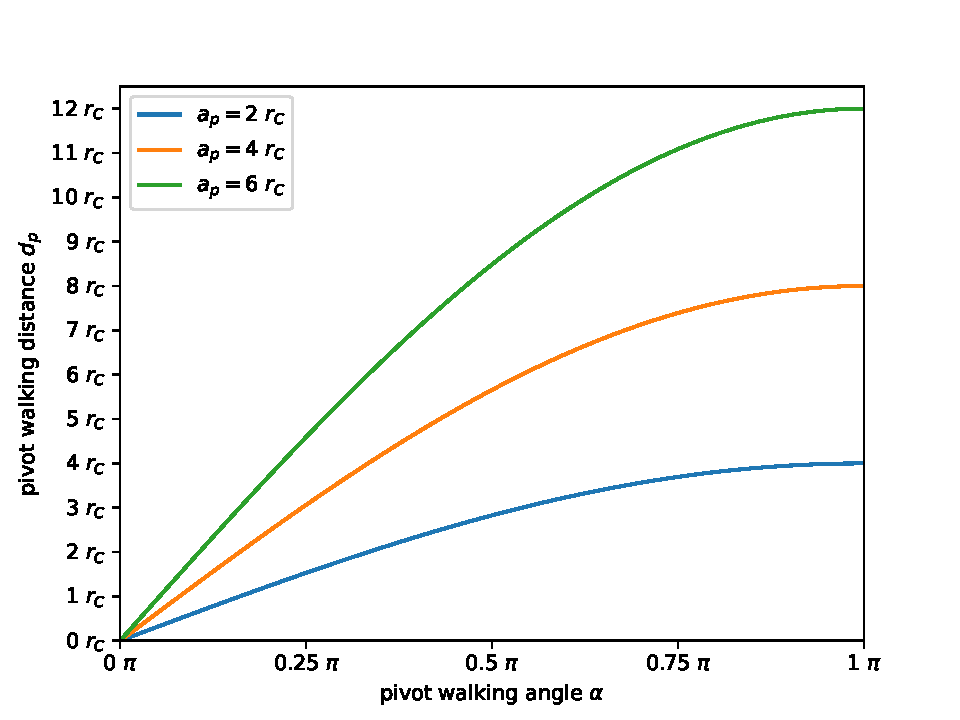
\includegraphics[width=0.60\textwidth]{figures/plots/pivot_walking_angle.pdf}
	\caption[Functions of $d_p$ based on $\alpha$ for different $a_p$]{Functions of the pivot walking distance $d_p$ based on pivot walking angle $\alpha$ for different pivot walking axes with length $a_p$. Lengths are given in multiples of cube radius $r_C$.}
	\label{fig:pw_angle_plot}
\end{figure}

\begin{figure}
	\centering
	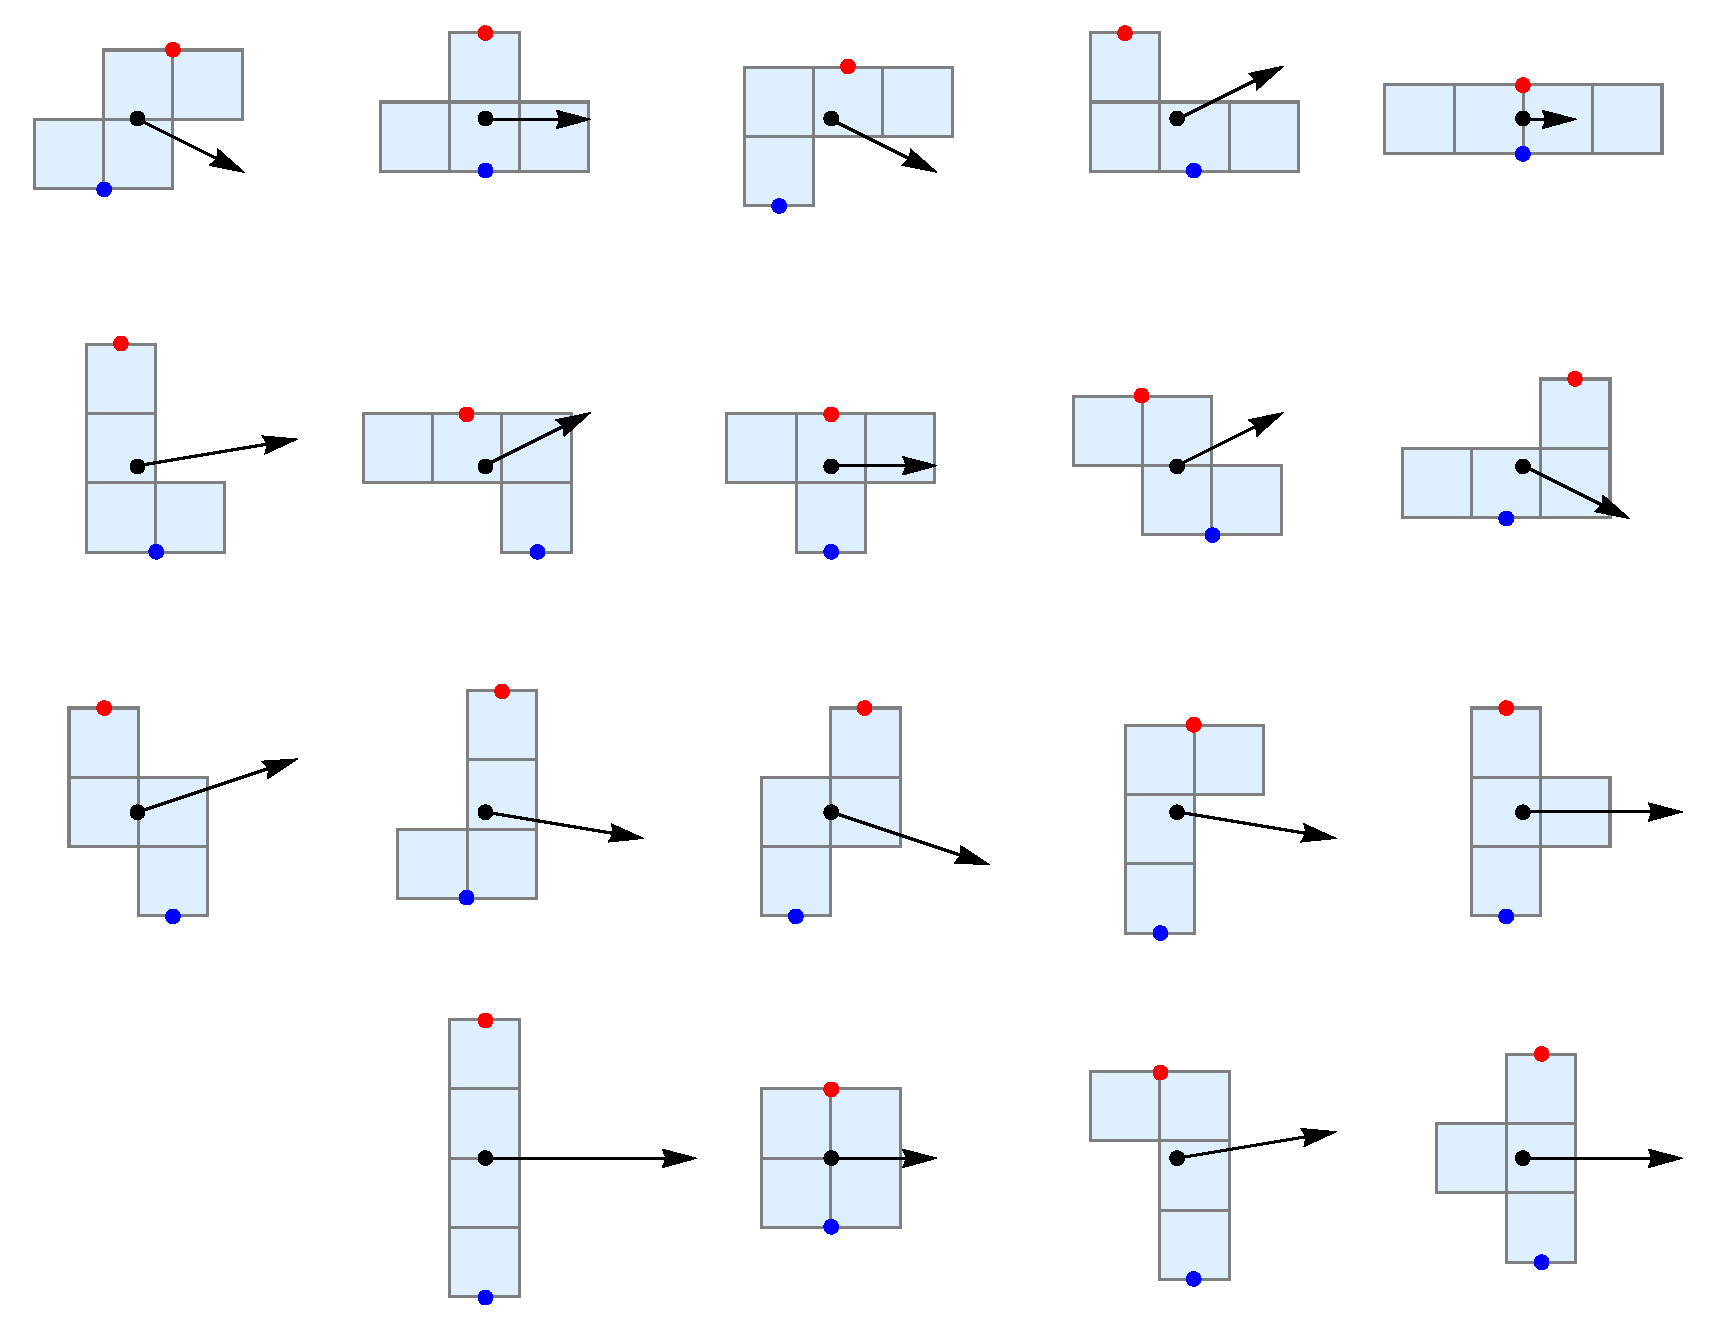
\includegraphics[width=0.70\textwidth]{figures/displacement_pivot_walking.pdf}
	\caption[Polyomino shapes with different displacement vectors]{All 19 four-cube polyomino shapes with their displacement vector $\vec{d}$ for one pivot walking cycle with $\alpha = \frac{\pi}{4}$. $\vec{d}$, drawn with a black arrow from its center of mass. North and south pivot point are drawn as red and blue dots.}
	\label{fig:displacement_pivot_walking}
\end{figure}

Not rotating around the center of mass is important for pivot walking.
In the first step of a pivot waking cycle, the magnetic field is elevated to let the polyomino pivot on its north pivot edge.
As a second step a rotation of $-\frac{1}{2} \cdot \alpha$ is performed around the north pivot point.
$-\pi \leq \alpha \leq \pi$ is the pivot walking angle.
For step 3 and 4 the elevation changes to its opposite to perform a rotation of $\alpha$ around the south pivot point.
Step 5 and 6 are equal to 1 and 2 and will bring the polyomino back to its original orientation.
You can see the pivot walking cycle steps in \autoref{fig:pivot_walking} a) and have a closer look at its parameters in \autoref{fig:pivot_walking} c).

After one pivot walking cycle, the polyomino has moved by a displacement vector $\vec{d}$ with $\lVert \vec{d} \rVert = d_p$, so $d_p$ is the distance the polyomino moved.
The direction and length of $\vec{d}$ changes with the shape of the polyomino.
The movement is always perpendicular to the pivot walking axis $\vec{a}$ with $\lVert \vec{a} \rVert = a_p$, which is the vector between the north and the south pivot point, visualized in \autoref{fig:pivot_walking} b).
$d_p$ can be calculated as
\begin{equation}
d_p = 2 \cdot \sin\left(\frac{1}{2} \cdot \alpha \right) \cdot a_p \,.
\end{equation}
\autoref{fig:pw_angle_plot} shows functions for this equation based on $\alpha$ for different $a_p$.
To calculate $\vec{d}$ you can take the perpendicular of $\vec{a}$ and scale it to the length $d_p$.

When a big $\alpha$ is chosen according to amount, $d_p$ becomes also bigger, but the polyomino needs more space to the north and south to perform the rotations.
For better maneuvering smaller values of $\alpha$ are preferable.
There is a strong deviation of length and direction of the displacement for different polyomino shapes.
Doing a pivot walking motion might not move two polyominoes in the same direction.
\autoref{fig:displacement_pivot_walking} shows all 19 four-cube polyomino shapes with their displacement vectors.
There are still two options for pivot walking, depending on a negative or positive value of $\alpha$.
You can walk left, in the direction of the west-faces, or right, in the direction of the east-faces.
Although the polyomino actually moves in the direction of $\vec{d}$, we can still say that a pivot walk right moves to the east, because $\left| \angle \left( \vec{E}, \vec{d} \right) \right| < \frac{\pi}{2}$.
We call these two options the pivot walking direction $\vec{w} \in \{\vec{E}, \vec{W}\}$.

	
	\bibliographystyle{abbrv}
	\bibliography{bibliography.bib}

\end{document}